\subsection{Word Importance Estimation in Deep Learning Models}


\begin{figure}
 \begin{center}
  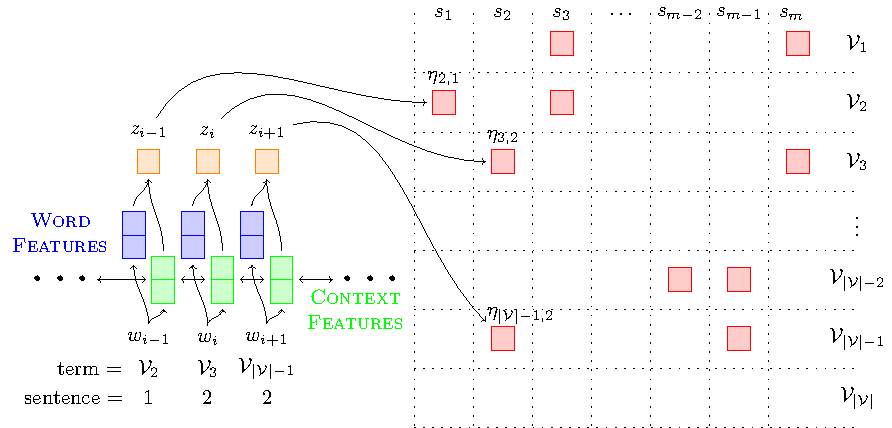
\includegraphics[scale=1.0]{dl_based_salience_models/figures/4_2_wimp_model.pdf}
 \end{center}
 \caption{(Left) Word and context features are extracted from the flat token
sequence representation to get word level importance scores 
$\wordImportance_i$. (Right) Word level scores are aggregated into a sparse
bag-of-words matrix with rows and columns corresponding to sentences and 
words respectively.}
\end{figure}

Our previous experiments revealed that lexical sematics were not the 
main driver of learning in sentence extractive news summarization. 
One could plausibly argue that it is a feature, not a bug, and that 
the structural
signals in news are intentional and not to be avoided. However, we think more 
attention could be paid to estimating importance scores at the word level.
We are motivated by potential application to abstractive generation: better
word level importance estimation could help to remove all but the most 
necessary content from the documents as a preprocessing stage before
abstractive summarization. We are also encouraged by practices
in multi-document news summarization, where word importance weights 
are the main ingredient in sentence representations. 


\newcommand{\classy}{\textsc{Classy}}
\newcommand{\occams}{\textsc{Occams}}

%\subsubsection{A brief discussion of \mlingsys.}

\occams{} and its antecedent \classy{} have been consistent top performers in various
summarization workshops \citep{conroyback,conroyclassy,davis2012occams}. 
In general their main approach 
is to represent each sentence as a sparse bag-of-words, where non-zero
entries correspond to word importance weights for the words found in the 
sentence. Typically, tf-idf weights are used for the importance scores.
The term by sentence matrix representing the document or documents to be
summarized is then factorized into two  matrices (typically with
non-negative entries) representing term factors and sentence factors.
The entries in the sentence factor matrix represent latent ``topics,'' 
and apriori the importance of each sentence is the sum of its latent topic
entries.

Sentence selection can subsequently be performed using one of several methods.
In the naive case, one can select the sentence with the highest vector norm, 
substract the selected latent factors from the remaining sentence vectors
(zeroing out any terms that become negative), and repeating until the
summary length budget is reached. More sophisticated selection procedures
involving multi-dimensional knapsack packing or submodular optimization 
can be used, however these are not the focus of this work.

One draw back to this approach is that the sentence factors and word 
importance scores are unsupervised with respect to the final summarization
objective; their utility to the summarization task is a happy coincidence.
Additionally, the word importance scores are not assigned based on the 
context in which the word appears.

We propose to address these issues by learning word level importance 
scores in the process of single document sentence extractive summarization.
Additionally, we propose a method of adapting these scores from the 
single document case to multi-document summarization.

\subsubsection{Proposed Model}


%In our proposed model for word importance, we first run the \elmo{}model 
%\citep{peters2018deep}
%over the input document to obtain contextual representations
%of each word. The \elmo{}embeddings are then combined with pretrained
%\glove embeddings along with embeddings for document frequency, 
%topic signature,
%sentence position, and part-of-speech tag, and then
%fed into a multi-layer perceptron to predict a scalar importance score.
%When a word occurs multiple times in the input, it can be given a different 
%importance score at each location because the \elmo{} embeddings will capture
%contributions of the salient neighbor words. A term-sentence matrix is 
%then formed from the input, using the estimated word importance scores 
%as the term weights. A sentence extractive summary can be obtained 
%using the naive sentence selection method described above or in 
%\autoref{alg:wimp_ext_alg}.
%The total score for the summary can also be obtained.
%
%We can train this summarizer using a gold extract sequence and a margin loss
%\[\objective(\theta) = \max\big(0, 1 + f(\predSaliences; \theta) - f(\saliences; \theta) \big) \] where $f(\predSaliences;\theta)$ is
%the score of our predicted extract summary.
%
%
%Let $\bowvec_1, \bowvec_2, \dots, \bowvec_n$ be the bag of words 
%representations of the 
%sentences selected for the summary, in the order they were selected.
%The score for the summary is computed as computed by the simple selection
%procedure would be
%$f() = \sum_{i=1}^n \sum_{j=1}^k \max(0, z_{i,j} - \sum_{l=1}^{i-1} z_{l,j})$ 
%
%
%~\\
%~\\

Let $\vocab$ be a finite vocabulary of words. A document $\doc$
is a sequence of $m$ words $(\word_1, \word_2, \ldots, \word_m) \in \vocab^m$.
We define two mappings of words to dense vector representations.
The first $\fdef{\wordFeatures}{\vocab}{\Rn{n_f}}$ maps words to 
a concatenation of feature embeddings whose total dimension is of size $n_f$. 
The various components of the feature embeddings include the word's \glove{} 
embedding, as well as embeddings for sentence position, document frequency,
and other word features that have been shown to be useful for summarization.
The second mapping
$\fdef{\contextFeatures}{\vocab}{\Rn{n_c}}$ maps the word to it's contextual
embedding; here this corresponds to the output of \elmo{} 
\citep{peters2018deep} at that word's
position in the document. 
The importance score $\wordImportance_i$ of a word $\word_i$ is the output of 
a feedforward layer 
\[ \wordImportance_i = \sigma\Big(\mathbf{v}^T \left[\begin{array}{c} \wordFeatures(\word_i) \\ \contextFeatures(\word_i) \end{array} \right] + b \Big) \]
    where $\mathbf{v} \in \Rn{n_f + n_c}$ and $b \in \R$ are learned weight
and bias parameters, and $\sigma$ is the logistic sigmoid.

Next, we aggregate the flat token level scores $\wordImportance_i$ into a
bag-of-words (BOW) 
representation for each sentence in the document.
Let $I_i$ be the set of indices of the flat word sequence corresponding
to the words in $i$-th input sentence. Then, let $\bow_i$ be the BOW 
representation of the $i$-th sentence with entries 
\[ \bow_{i,j} = \begin{cases} 
    0 & \textrm{if $\word_k \ne \vocab_j $ for all $k \in I_i $} \\ 
\sum_{k \in I_i} \mathbbm{1}\{\word_k = \vocab_j \} \cdot \wordImportance_k  & \textrm{otherwise}     \end{cases} \]
        for all $j \in \{1, \ldots, |\vocab|\}$.



\begin{figure}
  \begin{algorithmic}[1]
      \Procedure{\textsc{BowExtracter}}{$\bow_{1:n}, \beta, \kappa$}
   
      \State $\bow_i^{(1)}  \gets \bow_i \quad \forall i \in \{1, \ldots, n\}$
      \State $\hat{\eta} \gets 0$
      \State $t \gets 0$
      \While{ $\sum_{i=1}^t \kappa_{\predLabels_i} < \beta$ and $t < n$}
        \State $t \gets t + 1$
        \State $\predLabels_t \gets \operatorname{arg max}_{i \in \{1,\ldots, n\}}
            \sum_{j=1}^{|\vocab|} \bow^{(t)}_{i,j}$
            \State $\bow_i^{(t+1)} \gets \max(0, \bow_i^{(t)} - \bow^{(t)}_{\predLabels_t} )\quad  \forall i \in \{1, \ldots, n \}$
        \State $\hat{\eta} \gets \hat{\eta} + \sum_{j=1}^{|\vocab|} \bow_{\predLabels_t,j}^{(t)}$
         

      \EndWhile
        \State \Return $[\predLabels_1,\ldots,\predLabels_t], \hat{\eta}$ \Comment{Returns summary sentence indices and summary score.}
    \EndProcedure
  \end{algorithmic}
\caption{Simple sentence extraction algorithm given
 the sentence BOW representations $\omega_i$, 
  a word budget $\beta$, and a vector $\kappa$ of sentence lengths (in words)
  as input.}
\label{alg:wimp_ext_alg}
\end{figure}



        With the BOW representations in hand, we perform sentence selection
        using the algorithm presented in \autoref{alg:wimp_ext_alg} to 
        obtain a predicted extract indices $\predLabels$ and their associated
        overall summary score $\hat{\eta}$.

        We can optimize this model using a margin loss, where given a 
        gold extract sequence  $\labels$, we can compute the associated
        gold extract summary score $\eta$ and then minimize the following
        loss function \[\mathcal{L}_{ext}(\predLabels, \labels;\theta) = \max\big(0, 1 + \hat{\eta} - \eta\big)\]
        with respect to the parameters $\theta$ of the word importance 
        predictor.
        If needed, we can also introduce a supervised learning signal to the 
        individual word importance scores by collecting labels $\zeta_i$ for
        each $\wordImportance_i$ such that $\zeta_i = 1$ if $\word_i$ occurs
        and any human reference abstract and $0$ otherwise. The 
        $\objective_{ext}$ would then be augmented with an additional cross
        entropy loss for the word level predictions:
        \[ \mathcal{L}_{word}(\wordImportance, \zeta; \theta) = -\sum_{i=1}^m \zeta_i \log \wordImportance_i + (1 - \zeta_i) \log (1 - \wordImportance_i). \] 




        \paragraph{Adaptation to MDS} We also propose a simple 
        self attention-based modification to
        the word importance aggregation step to help adapt this method
        to multi-document summarization (MDS). \cite{conroy2013multilingual} 
        found
        that dimensionality reduction on the BOW representations improves
        summarizer performance in the MDS setting (but not as much on
 single document
        summarization). 


        We plan to experiment with the following importance 
        aggregation method. First, given the outputs of the contextual features
        $\mathbf{h}_i = \contextFeatures(\word_i)$, 
        we compute a self attention matrix $\Lambda \in \Rn{m\times m}$
        where \[\Lambda_{i,j} = \sigma(\mathbf{h}_i^T \mathbf{h}_j / \tau + b)  \]
        using sigmoidal attention \citep{kim2017structured} with a learned bias 
        parameter $b$ and a temperature parameter $\tau$.
        Next we compute an attention weighted word importance score $\bar{\wordImportance}_i$ for each word in the input using the following formula,
        \[ \bar{\wordImportance}_i = \sum_{j=1}^m \wordImportance_j \cdot \Lambda_{i,j}.\]
        We then use the aggregated word importance scores 
    $\bar{\wordImportance}_i$ inplace of their nonaggregated counterparts
        in the creating the BOW representations $\omega_j$.

        Our motivation is that by accumulating scores based on context
        similarity, words and topics that appear in multiple documents 
        will accumulate the bulk of the word importance scores, giving 
        an added boost to sentences that contain them. Implicitly, errant
        words from one document that are not on topic to the cluster will
        effectively not contribute much to a sentences score, reducing the 
        effectve dimension of the BOW vectors and regularizing individual
        sentences to the document cluster's mean.

        
        Since we are training our models on single documents, we expect that
        running our pretrainined word scoring model on the individual 
        documents from an MDS document cluster will result in 
        minimal task-adaptation mismatch. The remaining bias and temperature
        parameters can easily be tuned on the small amount of MDS training 
        data available.

%        We also plan to compare this method to using a non-negative matrix 
%        factorization 
%        method on the output of the learned BOW representation, 
%        and to hard attention assignments using Brown clustering.







%\subsubsection{
%\cite{conroy} 


 
